% Created by tikzDevice version 0.8 on 2015-01-07 01:15:39
% !TEX encoding = UTF-8 Unicode
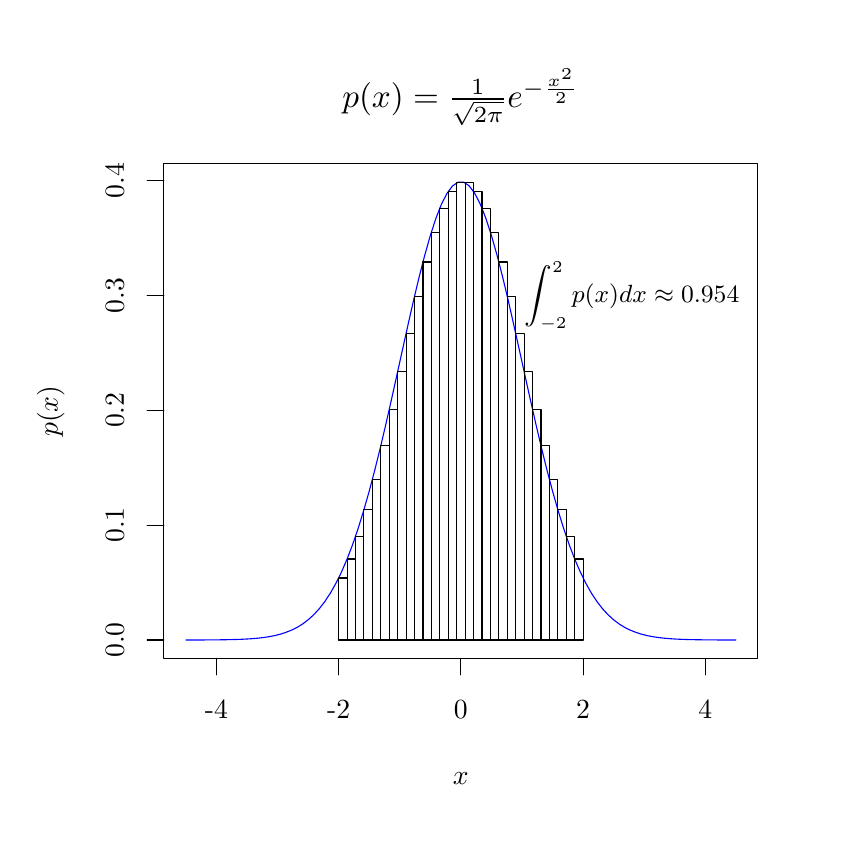
\begin{tikzpicture}[x=1pt,y=1pt]
\definecolor{fillColor}{RGB}{255,255,255}
\path[use as bounding box,fill=fillColor,fill opacity=0.00] (0,0) rectangle (289.08,289.08);
\begin{scope}
\path[clip] ( 49.20, 61.20) rectangle (263.88,239.88);
\definecolor{drawColor}{RGB}{0,0,255}

\path[draw=drawColor,line width= 0.4pt,line join=round,line cap=round] ( 57.15, 67.82) --
	( 59.16, 67.82) --
	( 61.17, 67.83) --
	( 63.17, 67.83) --
	( 65.18, 67.84) --
	( 67.19, 67.86) --
	( 69.20, 67.88) --
	( 71.21, 67.91) --
	( 73.21, 67.95) --
	( 75.22, 68.00) --
	( 77.23, 68.07) --
	( 79.24, 68.17) --
	( 81.25, 68.31) --
	( 83.25, 68.48) --
	( 85.26, 68.72) --
	( 87.27, 69.02) --
	( 89.28, 69.41) --
	( 91.28, 69.92) --
	( 93.29, 70.56) --
	( 95.30, 71.36) --
	( 97.31, 72.35) --
	( 99.32, 73.58) --
	(101.32, 75.09) --
	(103.33, 76.91) --
	(105.34, 79.09) --
	(107.35, 81.68) --
	(109.36, 84.72) --
	(111.36, 88.26) --
	(113.37, 92.33) --
	(115.38, 96.98) --
	(117.39,102.22) --
	(119.39,108.07) --
	(121.40,114.53) --
	(123.41,121.58) --
	(125.42,129.18) --
	(127.43,137.28) --
	(129.43,145.80) --
	(131.44,154.65) --
	(133.45,163.70) --
	(135.46,172.83) --
	(137.47,181.88) --
	(139.47,190.68) --
	(141.48,199.08) --
	(143.49,206.90) --
	(145.50,213.97) --
	(147.50,220.14) --
	(149.51,225.26) --
	(151.52,229.21) --
	(153.53,231.90) --
	(155.54,233.26) --
	(157.54,233.26) --
	(159.55,231.90) --
	(161.56,229.21) --
	(163.57,225.26) --
	(165.58,220.14) --
	(167.58,213.97) --
	(169.59,206.90) --
	(171.60,199.08) --
	(173.61,190.68) --
	(175.61,181.88) --
	(177.62,172.83) --
	(179.63,163.70) --
	(181.64,154.65) --
	(183.65,145.80) --
	(185.65,137.28) --
	(187.66,129.18) --
	(189.67,121.58) --
	(191.68,114.53) --
	(193.69,108.07) --
	(195.69,102.22) --
	(197.70, 96.98) --
	(199.71, 92.33) --
	(201.72, 88.26) --
	(203.72, 84.72) --
	(205.73, 81.68) --
	(207.74, 79.09) --
	(209.75, 76.91) --
	(211.76, 75.09) --
	(213.76, 73.58) --
	(215.77, 72.35) --
	(217.78, 71.36) --
	(219.79, 70.56) --
	(221.80, 69.92) --
	(223.80, 69.41) --
	(225.81, 69.02) --
	(227.82, 68.72) --
	(229.83, 68.48) --
	(231.83, 68.31) --
	(233.84, 68.17) --
	(235.85, 68.07) --
	(237.86, 68.00) --
	(239.87, 67.95) --
	(241.87, 67.91) --
	(243.88, 67.88) --
	(245.89, 67.86) --
	(247.90, 67.84) --
	(249.91, 67.83) --
	(251.91, 67.83) --
	(253.92, 67.82) --
	(255.93, 67.82);
\end{scope}
\begin{scope}
\path[clip] (  0.00,  0.00) rectangle (289.08,289.08);
\definecolor{drawColor}{RGB}{0,0,0}

\path[draw=drawColor,line width= 0.4pt,line join=round,line cap=round] ( 68.19, 61.20) -- (244.89, 61.20);

\path[draw=drawColor,line width= 0.4pt,line join=round,line cap=round] ( 68.19, 61.20) -- ( 68.19, 55.20);

\path[draw=drawColor,line width= 0.4pt,line join=round,line cap=round] (112.37, 61.20) -- (112.37, 55.20);

\path[draw=drawColor,line width= 0.4pt,line join=round,line cap=round] (156.54, 61.20) -- (156.54, 55.20);

\path[draw=drawColor,line width= 0.4pt,line join=round,line cap=round] (200.71, 61.20) -- (200.71, 55.20);

\path[draw=drawColor,line width= 0.4pt,line join=round,line cap=round] (244.89, 61.20) -- (244.89, 55.20);

\node[text=drawColor,anchor=base,inner sep=0pt, outer sep=0pt, scale=  1.00] at ( 68.19, 39.60) {-4};

\node[text=drawColor,anchor=base,inner sep=0pt, outer sep=0pt, scale=  1.00] at (112.37, 39.60) {-2};

\node[text=drawColor,anchor=base,inner sep=0pt, outer sep=0pt, scale=  1.00] at (156.54, 39.60) {0};

\node[text=drawColor,anchor=base,inner sep=0pt, outer sep=0pt, scale=  1.00] at (200.71, 39.60) {2};

\node[text=drawColor,anchor=base,inner sep=0pt, outer sep=0pt, scale=  1.00] at (244.89, 39.60) {4};

\path[draw=drawColor,line width= 0.4pt,line join=round,line cap=round] ( 49.20, 67.81) -- ( 49.20,233.87);

\path[draw=drawColor,line width= 0.4pt,line join=round,line cap=round] ( 49.20, 67.81) -- ( 43.20, 67.81);

\path[draw=drawColor,line width= 0.4pt,line join=round,line cap=round] ( 49.20,109.33) -- ( 43.20,109.33);

\path[draw=drawColor,line width= 0.4pt,line join=round,line cap=round] ( 49.20,150.84) -- ( 43.20,150.84);

\path[draw=drawColor,line width= 0.4pt,line join=round,line cap=round] ( 49.20,192.36) -- ( 43.20,192.36);

\path[draw=drawColor,line width= 0.4pt,line join=round,line cap=round] ( 49.20,233.87) -- ( 43.20,233.87);

\node[text=drawColor,rotate= 90.00,anchor=base,inner sep=0pt, outer sep=0pt, scale=  1.00] at ( 34.80, 67.81) {0.0};

\node[text=drawColor,rotate= 90.00,anchor=base,inner sep=0pt, outer sep=0pt, scale=  1.00] at ( 34.80,109.33) {0.1};

\node[text=drawColor,rotate= 90.00,anchor=base,inner sep=0pt, outer sep=0pt, scale=  1.00] at ( 34.80,150.84) {0.2};

\node[text=drawColor,rotate= 90.00,anchor=base,inner sep=0pt, outer sep=0pt, scale=  1.00] at ( 34.80,192.36) {0.3};

\node[text=drawColor,rotate= 90.00,anchor=base,inner sep=0pt, outer sep=0pt, scale=  1.00] at ( 34.80,233.87) {0.4};

\path[draw=drawColor,line width= 0.4pt,line join=round,line cap=round] ( 49.20, 61.20) --
	(263.88, 61.20) --
	(263.88,239.88) --
	( 49.20,239.88) --
	( 49.20, 61.20);
\end{scope}
\begin{scope}
\path[clip] (  0.00,  0.00) rectangle (289.08,289.08);
\definecolor{drawColor}{RGB}{0,0,0}

\node[text=drawColor,anchor=base,inner sep=0pt, outer sep=0pt, scale=  1.00] at (156.54, 15.60) {$x$};

\node[text=drawColor,rotate= 90.00,anchor=base,inner sep=0pt, outer sep=0pt, scale=  1.00] at ( 10.80,150.54) {$p(x)$};
\end{scope}
\begin{scope}
\path[clip] ( 49.20, 61.20) rectangle (263.88,239.88);
\definecolor{drawColor}{RGB}{0,0,0}

\path[draw=drawColor,line width= 0.4pt,line join=round,line cap=round] (112.37, 90.23) --
	(115.41, 90.23) --
	(115.41, 97.07) --
	(118.46, 97.07) --
	(118.46,105.28) --
	(121.51,105.28) --
	(121.51,114.88) --
	(124.55,114.88) --
	(124.55,125.84) --
	(127.60,125.84) --
	(127.60,138.00) --
	(130.65,138.00) --
	(130.65,151.11) --
	(133.69,151.11) --
	(133.69,164.80) --
	(136.74,164.80) --
	(136.74,178.62) --
	(139.78,178.62) --
	(139.78,192.02) --
	(142.83,192.02) --
	(142.83,204.41) --
	(145.88,204.41) --
	(145.88,215.22) --
	(148.92,215.22) --
	(148.92,223.87) --
	(151.97,223.87) --
	(151.97,229.93) --
	(155.02,229.93) --
	(155.02,233.04) --
	(158.06,233.04) --
	(158.06,233.04) --
	(161.11,233.04) --
	(161.11,229.93) --
	(164.16,229.93) --
	(164.16,223.87) --
	(167.20,223.87) --
	(167.20,215.22) --
	(170.25,215.22) --
	(170.25,204.41) --
	(173.30,204.41) --
	(173.30,192.02) --
	(176.34,192.02) --
	(176.34,178.62) --
	(179.39,178.62) --
	(179.39,164.80) --
	(182.43,164.80) --
	(182.43,151.11) --
	(185.48,151.11) --
	(185.48,138.00) --
	(188.53,138.00) --
	(188.53,125.84) --
	(191.57,125.84) --
	(191.57,114.88) --
	(194.62,114.88) --
	(194.62,105.28) --
	(197.67,105.28) --
	(197.67, 97.07) --
	(200.71, 97.07) --
	(200.71, 90.23);

\path[draw=drawColor,line width= 0.4pt,line join=round,line cap=round] (112.37, 67.81) --
	(200.71, 67.81);

\path[draw=drawColor,line width= 0.4pt,line join=round,line cap=round] (112.37, 67.81) -- (112.37, 90.23);

\path[draw=drawColor,line width= 0.4pt,line join=round,line cap=round] (115.41, 67.81) -- (115.41, 97.07);

\path[draw=drawColor,line width= 0.4pt,line join=round,line cap=round] (118.46, 67.81) -- (118.46,105.28);

\path[draw=drawColor,line width= 0.4pt,line join=round,line cap=round] (121.51, 67.81) -- (121.51,114.88);

\path[draw=drawColor,line width= 0.4pt,line join=round,line cap=round] (124.55, 67.81) -- (124.55,125.84);

\path[draw=drawColor,line width= 0.4pt,line join=round,line cap=round] (127.60, 67.81) -- (127.60,138.00);

\path[draw=drawColor,line width= 0.4pt,line join=round,line cap=round] (130.65, 67.81) -- (130.65,151.11);

\path[draw=drawColor,line width= 0.4pt,line join=round,line cap=round] (133.69, 67.81) -- (133.69,164.80);

\path[draw=drawColor,line width= 0.4pt,line join=round,line cap=round] (136.74, 67.81) -- (136.74,178.62);

\path[draw=drawColor,line width= 0.4pt,line join=round,line cap=round] (139.78, 67.81) -- (139.78,192.02);

\path[draw=drawColor,line width= 0.4pt,line join=round,line cap=round] (142.83, 67.81) -- (142.83,204.41);

\path[draw=drawColor,line width= 0.4pt,line join=round,line cap=round] (145.88, 67.81) -- (145.88,215.22);

\path[draw=drawColor,line width= 0.4pt,line join=round,line cap=round] (148.92, 67.81) -- (148.92,223.87);

\path[draw=drawColor,line width= 0.4pt,line join=round,line cap=round] (151.97, 67.81) -- (151.97,229.93);

\path[draw=drawColor,line width= 0.4pt,line join=round,line cap=round] (155.02, 67.81) -- (155.02,233.04);

\path[draw=drawColor,line width= 0.4pt,line join=round,line cap=round] (158.06, 67.81) -- (158.06,233.04);

\path[draw=drawColor,line width= 0.4pt,line join=round,line cap=round] (161.11, 67.81) -- (161.11,229.93);

\path[draw=drawColor,line width= 0.4pt,line join=round,line cap=round] (164.16, 67.81) -- (164.16,223.87);

\path[draw=drawColor,line width= 0.4pt,line join=round,line cap=round] (167.20, 67.81) -- (167.20,215.22);

\path[draw=drawColor,line width= 0.4pt,line join=round,line cap=round] (170.25, 67.81) -- (170.25,204.41);

\path[draw=drawColor,line width= 0.4pt,line join=round,line cap=round] (173.30, 67.81) -- (173.30,192.02);

\path[draw=drawColor,line width= 0.4pt,line join=round,line cap=round] (176.34, 67.81) -- (176.34,178.62);

\path[draw=drawColor,line width= 0.4pt,line join=round,line cap=round] (179.39, 67.81) -- (179.39,164.80);

\path[draw=drawColor,line width= 0.4pt,line join=round,line cap=round] (182.43, 67.81) -- (182.43,151.11);

\path[draw=drawColor,line width= 0.4pt,line join=round,line cap=round] (185.48, 67.81) -- (185.48,138.00);

\path[draw=drawColor,line width= 0.4pt,line join=round,line cap=round] (188.53, 67.81) -- (188.53,125.84);

\path[draw=drawColor,line width= 0.4pt,line join=round,line cap=round] (191.57, 67.81) -- (191.57,114.88);

\path[draw=drawColor,line width= 0.4pt,line join=round,line cap=round] (194.62, 67.81) -- (194.62,105.28);

\path[draw=drawColor,line width= 0.4pt,line join=round,line cap=round] (197.67, 67.81) -- (197.67, 97.07);

\path[draw=drawColor,line width= 0.4pt,line join=round,line cap=round] (200.71, 67.81) -- (200.71, 90.23);
\end{scope}
\begin{scope}
\path[clip] (  0.00,  0.00) rectangle (289.08,289.08);
\definecolor{drawColor}{RGB}{0,0,0}

\node[text=drawColor,anchor=base,inner sep=0pt, outer sep=0pt, scale=  1.20] at (156.54,260.34) {\bfseries $p(x)=\frac{1}{\sqrt{2\pi}}e^{-\frac{x^2}{2}}$};
\end{scope}
\begin{scope}
\path[clip] ( 49.20, 61.20) rectangle (263.88,239.88);
\definecolor{drawColor}{RGB}{0,0,0}

\node[text=drawColor,anchor=base,inner sep=0pt, outer sep=0pt, scale=  1.00] at (218.38,189.86) {\small$\displaystyle\int_{-2}^{2}p(x)dx\approx0.954$};
\end{scope}
\end{tikzpicture}
